\documentclass[11pt]{article} 
% The Proposal and Award Policies and Procedures Guide
% (PAPPG: https://www.nsf.gov/publications/pub_summ.jsp?ods_key=pappg)
% mandates, in Chapter 2, section B.2, that the main text should have a font size no less
% than 11 points for *most* typefaces (including Computer Modern Roman and Times (new) Roman).
% 
% Actually, Helvetica (a.k.a. Arial), Palatino and Courier New can drop
% to 10 point font size, according to the PAPPG, but be aware:
% 10-point fonts (whatever the typeface) will promote reader fatigue.
% Reader fatigue never works to the author's advantage.
%
%
% This sample  assumes the pdflatex chain (not the traditional latex | dvips | ps2pdf chain).
% It should function in the traditional chain if you comment out the hyperref package lines.
% 
% \usepackage{times} % uncomment for Times Roman;
%                   % replace "times" with other font names, as desired. 
\usepackage{bm} % If you want bold math, but without the bloat of AMS packages
\usepackage{color} % doh
\usepackage{hyperref} % LaTeX cross references become hyperlinks in pdf output
\usepackage{graphicx} % For figure insertion
\usepackage{vmargin} % To set page size

\usepackage{titlesec}
% \usepackage[T1]{fontenc}
% \usepackage{lmodern}
\usepackage{times}
% \fontsize{11.5}{12.6}\selectfont

\usepackage{amssymb}
\usepackage{float}
\usepackage{wrapfig}

\usepackage[svgnames,x11names,table]{xcolor}
\usepackage{hyperref}
\usepackage{enumitem}

\usepackage{subcaption}
\hypersetup{colorlinks,linkcolor={black},citecolor={black}} 

\usepackage{svg}
\newtheorem{definition}{Definition}

\usepackage{amsfonts, amssymb, amsmath, amsthm, euscript}
\usepackage{soul}
\usepackage{mathabx}
\usepackage{mathtools}
\mathtoolsset{showonlyrefs}

\usepackage[utf8]{inputenc}
\usepackage[margin=0.6in]{geometry}
\usepackage{tabularx}
\usepackage{booktabs}
\usepackage[table]{xcolor}
\usepackage{ragged2e}

% Color Definitions from Source
\definecolor{secprop}{HTML}{E8EDF5}
\definecolor{secowt}{HTML}{FDF3DF}
\definecolor{secopp}{HTML}{EEF6EE}
\definecolor{secoss}{HTML}{F0EDFF}

% Heatmap Colors
\definecolor{h5}{HTML}{1E4D2B} % Best
\definecolor{h4}{HTML}{2D7A45} 
\definecolor{h3}{HTML}{88C99E}
\definecolor{h2}{HTML}{C8E6D0}
\definecolor{h1}{HTML}{EAF5EE}
\definecolor{a3}{HTML}{5B4DBB} % Academic Best
%do before 
\input{utils/math-cmds}

\DeclareMathOperator{\mes}{\bm m}
\newcommand{\md}{\mathrm d}
\newcommand{\TV}{\mathrm{TV}}

\newcommand{\norm}[1]{\left\lVert#1\right\rVert}
\newcommand{\bx}{X}
\newcommand{\cE}{\mathcal{E}}
\newcommand{\PZ}{{\mathbb P_Z}}
\newcommand{\Pdata}{{\mathbb P_{\mathrm{data}}}}
\newcommand{\cL}{\mathcal{L}}
\newcommand{\cJ}{\mathcal{J}}
\newcommand{\cF}{\mathcal{F}}
\newcommand{\cD}{\mathcal{D}}
\newcommand{\cG}{\mathcal{G}}
\newcommand{\PP}{\mathbb{P}}
\newcommand{\RR}{\mathbb{R}}
\newcommand{\QQ}{\mathbb{Q}}
\newcommand{\cS}{\mathcal{S}}
\newcommand{\cH}{\mathcal{H}}
\newcommand{\cX}{\mathcal{X}}
\newcommand{\cY}{\mathcal{Y}}


\newcommand{\flowt}{t}      % Flow time (0 to 1)
\newcommand{\vidk}{k}       % Video frame index
\newcommand{\x}{\bm{x}}     % Data
\newcommand{\h}{\bm{h}}     % Latent state
\newcommand{\A}{\mathbf{A}} % State matrix
\newcommand{\B}{\mathbf{B}} % Input matrix
\newcommand{\C}{\mathbf{C}} % Output matrix
\newcommand{\D}{\mathbf{D}} % Feedthrough

\newcommand{\triplenorm}[1]{{\vert\kern-0.25ex\vert\kern-0.25ex\vert #1 
    \vert\kern-0.25ex\vert\kern-0.25ex\vert}}
\DeclareMathOperator{\Bin}{Bin}
\DeclareMathOperator{\Uni}{Uni}
\DeclareMathOperator{\Exp}{Exp}
\DeclareMathOperator{\Ave}{Ave}

\newcommand{\red}[1]{\textcolor{red}{#1}}
\newcommand{\blue}[1]{\textcolor{blue}{#1}}
\newcommand{\green}[1]{\textcolor{green!50!black}{#1}}

\newtheorem{theorem}{Theorem}[section]
\newtheorem{proposition}{Proposition}[section]
\newtheorem{lemma}{Lemma}[section]
\newtheorem{cor}{Corollary}[section]
%\theoremstyle{definition}
\newtheorem{assumption}{Assumption}
\newtheorem{example}{Example}[section]
\newtheorem{remark}{Remark}
\theoremstyle{definition}
\theoremstyle{remark}


\DeclareMathOperator*{\esssup}{ess\,sup}

\newcommand{\pseudodot}{{\lower 2.4pt\hbox{$\cdot$}}}
%
% Hyperref stuff: WARNING: don't use \href{link}{clickable text} in the Project Description,
% as Research.gov doesn't like it. Likewise, avoid any text containing 
% http:, https:, mailto:, etc.
%
\hypersetup{colorlinks=true,linkcolor=MidnightBlue,urlcolor=MidnightBlue}
%
% vmargin parameters:
% The Proposal and Award Policies and Procedures Guide
% (PAPPG: https://www.nsf.gov/publications/pub_summ.jsp?ods_key=pappg)
% mandates, in Chapter 2, section B.2, that margins must be at least 1 inch in all directions.
%
\setpapersize{USletter}
% \setmarginsrb{〈leftmargin〉}{〈topmargin〉}{〈rightmargin〉}{〈bottommargin〉}%{〈headheight〉}{〈headsep〉}{〈footheight〉}{〈footskip〉}
\setmarginsrb{1in}{1in}{1in}{1in}{0pt}{0mm}{0pt}{0mm}

%
% Pseudodot: break up "clickable" strings like "Data.gov" which you can
% enter as Data\pseudodot{}gov in your file.
% Use this trick in case research.gov misreads text such as "Data.gov" as a clickable hyperlink
% (even when it isn't).
%
%\def\pseudodot{{\lower 2.4pt\hbox{$\cdot$}}} %% This is the PlainTeX version.
%
% On with the show...
%
\begin{document}
\titlespacing*{\section}
{0ex}{3ex}{1.5ex}
\titlespacing*{\subsection}
{0ex}{2.5ex}{1.25ex}
\titlespacing*{\subsubsection}
{0ex}{2.5ex}{1ex}
%
% Remove page numbers---Research.gov will paginate the document instead
%
% \pagestyle{empty} 
%
% Line spacing: 
% The Proposal and Award Policies and Procedures Guide
% (PAPPG: https://www.nsf.gov/publications/pub_summ.jsp?ods_key=pappg)
% mandates, in Chapter 2, section B.2, that the main text should have no more than
% six lines to the vertical inch. With 72 points per inch, the minimum line skip 
% would be 12 points.
%
% \setlength{\baselineskip}{12.6pt} % in text mode
% \setlength{\normalbaselineskip}{12.6pt} % in math mode
\setlength{\parskip}{4pt}%

%%%%%%%%%%%%%%%%%%%%%%%%
% REMOVE/COMMENT
% \textbf{REMOVE BEFORE SUBMIT} \\
% \noindent\textbf{RI: Video Synthesis with Linear-Complexity Attention}  \\
% \textbf{TODO: leave out page numbering}
% \tableofcontents
\clearpage
%COMMENT out above before submission
%%%%%%%%%%%%%%%%%%%%%%%%%%%%%%%%
%Remove page number for submission
%%%%%%%%%%%%%%%%%%%%%%%%
% \pagestyle{empty}

% \setcounter{page}{1}
% \newpage
% \section*{RI: Video Synthesis with Linear-Complexity Attention}
\addcontentsline{toc}{section}{\protect\numberline{}Project Summary}


\subsection*{Project Overview: }
Large language models (LLMs) have demonstrated the transformative potential of generative artificial intelligence (AI), reshaping how people work, learn, and interact across domains such as engineering, education, and healthcare. At the core of what has enabled the generalization capabilities of a Agentic AI today is the autoregressive training of an LLM. In autoregressive training, text tokens up to a specific time point is used to predict subsequent tokens. We seek to study and build visual models in a similar way by training vision models using video instead of images alone. These types of linear-attention models were recently proposed to address the squared computational complexity of attention mechanisms. However, how they can be applied to work on video generation which is inherently multimodal, high-dimensional and along a long time series is not well understood. 

The primary focus of this proposal is to examine how to develop a generalized method for learning multimodal visual representations using linear-time attention over high-dimensional spatial data. Based on our preliminary work, there are a few technical challenges. For example, as the sequence length increases, the importance of samples seen from a long time ago decreases. How then should the features be ordered given this limitation? Furthermore, how should spatial from multiple modalities be linearized and fused?


In this RI proposal, we propose a synergestic set of enhancements to advance visual intelligence. We do this by improving the efficient learning of diffusion and flow-based models through novel architectural and framework advancements. 

\paragraph{Intellectual Merit} 
This work lies in merging the computational and foundational mathematical techniques to advance designing, evaluating, and optimizing multimodal video generation methods. First, the project proposes novel methods to replace the costly full attention mechanism in current state of the art diffusion-based video generation methods with linear-complexity alternatives. This model used to understand how we can incorporate autoregressive training in a visual model. Additionally we also propose  novel optimization techniques to enhance diffusion and flow-based model optimization of linear attention architectures to improve the quality and efficiency of video generation. This is extended into the multimodal setting by designing methods to fuse language and speech into a visual representation for conditional generation. Our work will be thoroughly verified according to machine learning best practices. Our source code along with weights will be open sourced following responsible AI use standards. 

\paragraph{Broader Impacts} 

The impact of an efficient video generation method is vast as it can lead to a generalizable vision model akin to the generalization capabilities of an LLM. If successful, our method can lead to new insights into physical intelligence which would enable robotic integration into daily life; it could also enable smarter and more personalized generation of multimodal tutoring and training content. The open source code of our computationally accessible method will be made available to scientists to support rapid prototyping of ideas which tackle pressing societal issues in education, health, and much more. Additionally, through the integration of our research into the curriculum, we create high-impact training opportunities for students at multiple institutions to prepare for critical workforce and national strategic needs outlined in America's AI Action Plan.

% \clearpage

\setcounter{page}{1}
\newpage
{\centering
{\Large \textbf{AutoDistill: Self-Training Small Reasoning Models for Efficient Generalization}} \\}
\vspace{0.5em}
\addcontentsline{toc}{section}{\protect\numberline{}Project Description}

\section{Introduction and Motivation}

The goal of this project is to develop effective and efficient deep learning algorithms for language, visual, and multimodal reasoning through distillation. Distillation is a form of transfer learning where a smaller specialized model is trained to replicate the behaviors of a larger model. Existing approaches to distillation utilize architectural~\textbf{CITE} and optimization~\textbf{CITE} methods to enable distillation for language~\textbf{CITE}, visual~\textbf{CITE}, and multimodal data~\textbf{CITE}. Traditionally, these methods have been applied to tasks such as language understanding, visual classification, and other tasks~\textbf{CITE}. However, there is an increasing indication that they should be extended to better support more complex reasoning and advanced artificial intelligence tasks. The technical need is important due to the proliferation of agentic systems. In addition to improving their efficient use, efficient methods to tune and adjust their behaviors are critically needed. 

Modern artificial intelligence (AI) and agentic systems fundamentally rely on a large language model or multimodal large language model. This is enabled through the use of a harness, which provides a software defined method to enable interaction with uesrs and the agent's environment. The harness then utilizes a LLM backend to reason, make predictions, and decide future actions based on the information and affordances provided by the agentic harness. Using this architecture, modern AI systems are demonstrating transformational capabilities in society. 

Popular benchmark tasks include language-controlled computer use, robotic manipulation, and others. However, due to the high computational and data costs associated with modifying a LLM backend, customizations are challenging and limited to techniques such as due to the computational and data requirements for running and modifying the LLM backend, at is core, agentic systems still rely on the foundational capabilities of the LLM.

Currently, the most performant LLMs are built using billions of parameters. On some tasks, they can exceed human performance \textbf{provide examples}. However, on many reasoning focused tasks, they do not perform as strongly \textbf{CITE}, performance benefits from scaling also appears to be plateauing \textbf{CITE}. Furthermore, due to their scale in terms of both data and compute requirements, training these models directly is out of reach for many researchers. Fortunately, there is evidence that small parameter models can solve problems that were initially only demonstrated on larger models. While there are certainly many factors which can lead to these observations, it indicates that parameter count is not the sole determinant of reasoning ability. The core goal of this proposal is to improve the intelligence\textbf{indirect} properties of LLMs without relying on scaling properties. 

To address this fundamental question, we propose to build small models with the same capabilities as larger models. We will tackle this by looking at distillation and understand how smaller models can replicate the capabilities of larger models. This will allow us to understand what are effective mechanisms, such as optimization or architectural enhancements, which enable this capability. This will enable us to develop new interpretable insights by understanding the effects that the proposed methods will have. Furthermore, the benefits of building smaller models will provide efficiency improvements for many resource-constrained compute settings. 




\section*{Intellectual Merit}

The proposed
The proposed foundational advancements in generative representation learning of multimodal video has transformative and far-reaching implications. For example, these models can be used in new vision-language-action models to benefit improved understanding of the physical world. This can support robotic (embodied or non-embodied) integration in society. By enabling integration, robots can help do household chores, support decision making, or automate mundane tasks. However, current large visual models are limited in their capabilities compared to large language models. For example, they cannot properly understand physical properties. In addition to these, video models are extremely expensive to train. In this proposal, we provide a potential solution towards addressing these issues. The goal is for the outcomes of our research to lead to broader scientific and interdisciplinary investigations into multimodal visual reasoning. 

We propose multiple innovations towards this goal. First, we extend existing diffusion and flow based generative methods to use lower complexity attention that is customized for video-based tasks. The attention mechanism in the network architecture is core to the what enables the algorithms of today and is extremely computationally expensive. Second, we take a first principles approach towards developing optimization methods for these diffusion and flow based methods. This will be used to enhance the learned representations in an improved and more computationally efficient manner. Lastly, we extend these efficient representation learning advancements into the multimodal domain to enable a foundational model that is trained and designed for multimodal understanding, reasoning, and use. Our work will be thoroughly verified according to machine learning best practices. Our source code along with weights will be open sourced following responsible AI use standards. 


\section{Background}


\noindent\textbf{Generative Models:} 
Generative models (i.e., deep learning models that can generate open-ended responses) have rapidly increased in usage recently, largely driven by LLMs \cite{zhang2024appagent, chen2025mlrbench}. High quality generative text models were first widely demonstrated by OpenAI's ChatGPT (which incorporated instruction tuning) \cite{ouyang2022training}. Generative models have grown beyond simple question answering to applications such as coding support \cite{dinh2023large, su-etal-2024-evor, shinn2023reflexion, wei2024magicoder, jimenez2024swebench}, complex task following \cite{wang2023voyager, zhang2024appagent, yu2025exact}, and conducting research \cite{chen2025mlrbench, gabriel2024advancing}. Newer generative models have started to incorporate visual and audio modalities. For example, they have been implemented to improve gaming frame rates \cite{li2024neural, mercier2023efficient, zhu2025generative}, upscale visuals \cite{xu2025videogigagan, zhou2024upscaleavideo, liu2025ultravsr}, and generate podcasts \cite{park2025speechssm}. A popular example in proposed morphing pixels to generate video from images (e.g., making a talking Mona Lisa) \cite{siarohin2019first}. 


\noindent\textbf{Attention:} The concept of attention in machine learning has been around for some time \cite{bahdanau2014neural} and was initially applied effectively on text datasets. This served as the foundation for the transformer architecture \cite{vaswani2017attention} that is widely used as a general feature extractor today. This simple intuition of how much to emphasize each feature vector, has served as the foundation for the AI advancements we see today in foundational models such as large language models (LLMs) and multimodal LLMs. In addition to their use in foundational models, special customizations and combinations with existing neutral architectures have been applied to many language, visual, and multimodal problems. 
Attention and transformers have been applied to multiple vision problems such as in image classification \cite{dosovitskiy2020vit} and action recognition \cite{nagrani2021attention}. The basic functionality is to apply layers of self-attention, on sequential representations. However, the a primary concern is its high computational complexity of $O(n^2)$. There have been several well-known works in developing a generalizable linear-complexity attention module. For example, \cite{katharopoulos2020transformers} examined how the attention mechanism is essentially similar to a similarity function and simplifies the computation in this manner. Mamba\cite{gu2023mamba}, also frequently referred to as State Space Model (SSM) attention, takes advantage of this and incorporates additional system level enhancements. These have also been applied to a variety of applications such as 3D vision \cite{ke2025mambev}.

\noindent\textbf{Knowledge Distillation: } Knowledge distillation approaches can be broadly categorized into off-policy and on-policy distillations. 
Standard methods generally operate via off-policy distillation, where the student learns from the teacher's logits on fixed, ground-truth datasets~\cite{hinton2015distilling,sanh2019distilbert,wu2024rethinking,kim2016sequence,wen2023f}.
While efficient, this setup suffers from exposure bias~\cite{arora2022exposure}, as the student never comes across its own incorrect generation during training.
Conversely, on-policy approaches~\cite{agarwal2024onpolicy,gu2024minillm,ko2024distillm,kodistillm} mitigate this training-inference mismatch by fine-tuning the student-generated output (SGO) sequences, but these methods suffer from self-generative inefficiency during training. Feature-based KD attempts to align the intermediate representations of the student and teacher directly. 
FitNets~\cite{romero2014fitnets} introduced regression losses to match the hidden states of intermediate layers. Subsequent works have proposed aligning attention maps~\cite{zagoruyko2017paying,wang2020minilm}.
Recently, works \cite{sun2019patient, gong2025beyond} proposed to distill the intermediate features from teacher to student using the asymmetric Kullback-Leibler divergence $\mathcal{L}_{KL}(p||q_\theta)$ metric, which undervalues the matching of low-probability regions.

\noindent\textbf{Efficient Machine Learning: } Distillation methods fall under 


\section{Research Plan}
\begin{table}[htbp]
    \centering
    \resizebox{\textwidth}{!}{
        \begin{tabular}{l l l c c c c c}
            \toprule
            \textbf{Company} & \textbf{Arch.} & \textbf{Size} & \textbf{Arena Elo} & \textbf{SWE-bench (\%)} & \textbf{MMMU Pro (\%)} & \textbf{MMLU Pro (\%)} & \textbf{GSM8K (\%)} \\
            \midrule
            
            \multicolumn{8}{c}{\textbf{Proprietary (Closed weights, closed source, API-only)}} \\
            \midrule
            Anthropic & Dense & Undisclosed & 1503 & 93.9 & 92.7 & 89.5 & 96.4 \\
            OpenAI & Dense & Undisclosed & 1488 & 88.7 & 94.0 & 92.5 & 97.1 \\
            Google & MoE & Undisclosed & 1493 & 80.6 & 83.9 & 91.0 & 86.2 \\
            Meta & Dense & Undisclosed & 1491 & 77.4 & 80.4 & -- & 77.7 \\
            \midrule
            
            \multicolumn{8}{c}{\textbf{Open Weights (Permissive and Restrictive)}} \\
            \midrule
            Alibaba / Qwen & MoE & 397B (17B act.) & -- & 76.2 & 86.0 & 88.5 & 95.9 \\
            MiniMax & MoE & 230B (10B act.) & -- & 80.2 & -- & 88.0 & -- \\
            DeepSeek & MoE & 1.6T (49B act.) & $\sim$1460 & 80.6 & -- & 87.5 & 95.1 \\
            Moonshot AI & MoE & $\sim$1T (32B act.) & $\sim$1460 & 80.2 & 79.4 & 87.1 & 97.3 \\
            Meta / Llama & MoE & 400B (17B act.) & -- & -- & 73.4 & 85.5 & -- \\
            Google / Gemma & Dense & 31B & -- & -- & 76.9 & 85.2 & 95.9 \\
            \midrule

            \multicolumn{8}{c}{\textbf{Fully Open Source (Weights + training scripts + datasets public)}} \\
            \midrule
            AllenAI / OLMo 2 & Dense & 32B & $\sim$1200 & -- & -- & $\sim$82.0 & 78.8 \\
            AllenAI / OLMoE & MoE & 7B (1B act.) & -- & -- & -- & $\sim$58.0 & 68.2 \\
            \bottomrule
        \end{tabular}
    }
    \caption{Comparison of open source and closed open weight models. A clear separation exists between their performance. . Values obtained from trackers and leaderboards.}
\end{table}

\noindent\textbf{PIs related prior work: } The proposed efforts directly leverage the PI's past work. PI Ding has conducted work on incorporating a Mamba-based method (one type of linear-attention method) into learning 3D representations~\cite{ke2025mambev} published at International Conference on Learning Representations. This also includes additional work~\cite{ke2025tinybev} and background in computer vision and machine learning~\cite{nishi2021augmentation,dhakal2026gft}. PIs have also done extensive work in the multimodal space~\cite{ding2019multimodal, ding2022impact, jinadu2024noise, mim2025can} and flow-based and differential-equation-related approaches \cite{celledoni2025mixed, yang2025finding} as well as the previously mentioned \cite{chen2023provably, hagemann2025multilevel, deng2024reflected, park2024dynamical, yang2026}.

\subsection{Thrust 1: Distillation}
Off-policy, On-Policy, dense to sparse, sample efficiency, multimodal, agentic distillation


\subsection{Aim 1: Efficient Intra-Family Distillation} 
This aim establishes a solid foundation to enable novel advancements to distillation methodology. We propose multiple advancements to the a constrained form of the distillation problem setup, which assumes that the teacher and student come from the same family. For example, distilling from a Llama model with 6.7B parameters to a 1.1B parameter Llama model. Distillation in such settings will help to improve the performance as well as improve model efficiency. Subsequent aims will relax this assumption to support additional enhancements. A canonical baseline approach for distillation typically involves three broad tasks. It is usually, but not necessarily, in order and can also be mixed with each other or partially skipped. First a strong teacher is chosen which is fine-tuned to a specific task of interest. Second, the teachers knowledge is transferred to the student. Lastly, additional fine-tuning is conducted on the student independent of the teacher. We discuss advancements and investigations for each of these components below.

\subsubsection{Weight initialization}
A baseline way to start the training of a neural network is to initialize the weights randomly~\cite{hinton2015distilling} or by training the student with an unsupervised objective~\cite{turc-etal-2020-well-read}.  However, this approach requires training the student model from scratch which requires a large amount of compute and is typically not used in practice except as a baseline comparison. Many works have explored how to initialize student weights based on teacher weights. For example, the student can copy a subset of the layers directly~\cite{wang-etal-2023-distill-bert, wang-etal-2023-distill-bert}. Another way to view this is through a pruning approach~\cite{xia-etal-2022-structured}. However, these approaches limit the adjustments possible such as requiring the similar latent space shape. Recently, it has been shown that it is possible to copy a subset of teacher layers as well as element weights to match a smaller student architecture during initialization~\cite{chen2024initializing}. This technique was demonstrated to be effective on visual features, therefore, an interesting research challenge remains on how similar approaches can be made to work with language features since they are fundamentally different in the representation space. Instead of selection based copying, factorization based methods enables a transformation into different representation dimensions~\cite{chen2021drone, ko2025efficient, yim2017gift, lee2018svd}. Distillation, however, is not limited to just creating a student which is smaller than a teacher model. Expanding model capacity has been demonstrated to be highly beneficial, several methods have explored how to widen or deepen a trained network. This can be done by expanding the width via random copying of neurons~\cite{chen2016net2net}, or by stacking multiple small models together~\cite{gong2019efficient}. The proposed work will examine how all these methods of initialization can interfere with the distillation process. For example, each initialization method introduces inductive biases into the student model. We will seek to understand how initialization can be improved to accelerate model training and to improve student model performance. 

\subsubsection{Student-teacher alignment}
Once the weights are initialized, the student will then learn to align its outputs with the teacher responses. This is typically done by defining an optimization objective to constrain the distance between the student and the teacher outputs. There are many forms of this distance, For example, the student can learn to align directly to the teacher's outputs via a cross-entropy loss:
\[
\mathcal{L}_{hard} = -\frac{1}{T}\sum_{t=1}^T \sum_{k=1}^K \tilde{y}^t_k \log p_s(k | x)
\]
where $\tilde{y}$ is a one-hot label from the teacher, and $k$ is the student output probability. This is also known as hard-label alignment~\cite{hinton2015distilling}, which is useful for example in settings where teacher logits are unavailable~\cite{wang2023self, taori2023stanford} or due to model structure differences~\cite{kim2016sequence}. However, using hard labels alone potentially requires a large amount of data to properly transfer knowledge~\cite{gudibande2023false}. To simplify the process, many works look at a slightly simpler approach where the teacher model logits are available for distillation. The logits provide a distribution over the possible outputs which can be aligned using Kullback-Liebler divergence or a L2 distance~\cite{ba2014deepnets}.
Many works focus on how we can most appropriately align the token distributions of the teacher and student. For example, analysis has looked at how forward KL loss tends to cover all modes of the distribution (i.e. mean seeking) which may be detrimental for the performance for small models~\cite{huszar2015not, gu2024minillm}.  Optimal transport based objectives can also be defined to support the knowledge transfer process.


If model weights are available, then the KD problem can be relaxed.  In addition to defining an optimization objective on the output layer, intermediate representation transfer can also help accelerate the representation learning process. Exploiting intermediate representations is useful for many reasons, for example, logit lens and linear probing techniques have long shown that intermediate layers provide interpretable value. Therefore, it would make sense to understand how this interpretability can benefit KD. The proposed work will explore how we can develop techniques to transfer intermediate layer dynamics and understanding during distillation. We will do this by understanding the latent data properties and look at how objectives and transformations 

\subsubsection{Post-distillation fine-tuning}

Once the knowledge transfer process from the teacher to student is complete, many techniques incorporate an additional fine-tuning process. For example, the student can be further fine-tuned on the task-specific dataset. Additionally, many generative or decoder-only models typically involve a RL fine tuning process to more specifically align task outputs to human preferences. However, in many scenarios, such preference tuning datasets may not be available. LLM-based preference feedback has been shown to be beneficial for this process where alignment data for specific tasks are unavailable. This LLM feedback can be incorporated into the tuning process via a DPO objective for example. A major challenge is that the feedback is noisy and can lead to hallucinations. We propose to look at how we can improve LLM-based feedback by accounting for noise. We will also look at how to reduce hallucinations by adding additional verification steps for the feedback signal. 

\subsection{Evaluation Methodology}
The dataset and evaluation methodology will be common to all proposed tasks. The discussion builds on Aim 1, but can be altered to suit the subsequent aims.

\subsubsection{Baseline methods} Our comparison spans standard, including Supervised Fine-Tuning (SFT) and Standard KD (Forward KL)~\cite{hinton2015distilling}, alongside Sequence-Level KD (SeqKD)~\cite{kim2016sequence}. 
To analyze the impact different loss formulations, we also benchmark against advanced divergence objectives: the mode-seeking Reverse KL (RKL), symmetric metrics like Jeffreys Divergence (JD)~\cite{jeffreys1948theory} and Jensen-Shannon Divergence (JSD), and the hybrid Adaptive KL (AKL)~\cite{wu2024rethinking}, which dynamically balances mean- and mode-seeking behaviors. We will also integrate our understanding derived from foundational evaluations into end-to-end approaches. We will also compare against a mix of on-policy and off-policy methods. In off-policy distillation, static sequences are first generated by a teacher. By optimizing on static sequences, these methods suffer from exposure bias~\cite{arora2022exposure}: a distribution mismatch arises because the model is trained on ground-truth sequences but evaluated on its own autoregressive generations~\cite{gu2024minillm}. 
This increased exposure bias directly degrades the generation capabilities of language models~\cite{arora2022exposure}. 
In contrast, on-policy distillation~\cite{gu2024minillm,agarwal2024onpolicy} mitigates this by training the student model $q_\theta$ on its own self-generated responses $y$ for given prompts $x$. 
However, this effectiveness comes at a high computational cost; the generation process introduces significant GPU overhead and slows down training~\cite{ko2024distillm,kodistillm}.

We will also compare our methods against framework-level or end-to-end methods such as MiniLLM, DistillLLM. \textbf{CITE}. We will also incorporate different LLMs into the training pipeline. We expect to perform most experiments using Gemma, Llama, Olmo, Qwen, Deepseek as these models have open weights. We will additionally incorporate closed source models such as those form OpenAI and Anthropic for evaluations, as feedback, and as real-world black-box evaluation. 

\subsubsection{Datasets}
Our evaluation spans five diverse benchmarks: a held-out \textbf{DollyEval} set (500 samples), the user-centric \textbf{SelfInst}~\cite{wang2023self}, and the reasoning-focused \textbf{VicunaEval}~\cite{zheng2023judging}. Additionally, we evaluate long-form generation capabilities using the  response subsets of \textbf{S-NI}~\cite{wang2022super} and \textbf{UnNI}~\cite{honovich2023unnatural}.


\subsubsection{Metrics}
We assess the quality of model-generated responses using Rouge-L (R-L)~\cite{lin2004rouge}. 
Prior studies~\cite{wang2022super} have demonstrated that Rouge-L correlates well with human evaluation for large-scale instruction-following tasks, making it a suitable proxy for measuring generation precision and recall against ground truth references.
We estimate the semantic similarity with the ground truth using GPT-4o-mini~\cite{hurst2024gpt} as the judge and the SBERT score using Sentence-BERT models~\cite{reimers2019sentence}.
The GPT-4o-mini evaluation prompts are modified from prior work~\cite{zheng2023judging}.

\subsection{Aim 2: Multimodal Large Language Model Distillation}
In this aim, we will explore how to distill MLLM models. Large language models 

\subsection{Aim X: Multitask distillation under data constraints}
There are many circumstances where we wish to preserve performance of multiple tasks or datasets. For example, it is beneficial to maintain safety guardrails of a model while improving task performance. We will investigate how we can do this. One naive approach is to use multiple datasets depending on the tasks of interest. In practice, not all data available for teacher models may be available for distillation. Therefore, naive approaches will be limited due to data availability uniformity. Additionally, it has been shown previously that prompt templates can have an impact on model performance~\textbf{CITE} which raises fundamental questions about the behavior of how models learn. We will examine how these training and optimization effects transfer into a distillation setting. We will analyze attention weights of different prompting and learning scenarios and create visualizations using t-SNE and other projection methods. We will explore methods of sample selection, augmentation, network customizations, and customized optimization objects can be used to overcome inductive biases in multitask distillation settings. 

The typical way in 

\subsubsection{Template mixing in distillation}

\subsubsection{Few-shot distillation}

\subsection{Aim X: Distillation across model families}
Distillation across families of models, for example from Qwen to Llama, is important since the models demonstrate superior capabilities on different tasks. However, transferring across model family is challenging for several major reasons:
\begin{itemize}
    \item Tokenizer mismatch: Tokenization is required part of the pipeline which breaks down raw data into chunks. These chunks can represent whole words. Qwen for example, uses BPE-based~\cite{qwenteam2025qwen3} tokenization, while Gemma uses SentencePiece~\cite{kudo2018sentencepiece} tokenization. 
    \item Vocabulary: Special tokens, such as templates, for each language model and accommodations for language (i.e. mandarin vs english) and task-specific optimizations can change the vocabulary size, and allocation. 
    \item Architectural choices: Even if architectures are aligned in using transformers, the hidden state, alyer counts, positional encoding, data and other factors all change the learned representation. This can be complicated by the use of different attention mechanisms~\cite{gu2023mamba, peng2023rwkv} or use of sparse mixture-of-experts models for example. 
    \item Policy: Policy choices in model training, such as what is considered safe or non-safe in responses, will need to be addressed during distillation. Where these boundaries lie creates complications in formulating an appropriate distillation objective.
\end{itemize}
The above provides a non-exhaustive list of possible challenges when conducting cross-family distillation. We will address these challenges and more in our investigations of cross-family distillation. This outcomes of this research aim will be to develop a fundamental understanding for how we can transfer knowledge across families of models. 

To tackle these problems, we will look at how intermediate and final output representations can be transformed. We will first do this through a rigorous unsupervised representation analysis of the data and corresponding representations. We will also examine and evaluate how theoretical understanding of representations can inform the design of novel distillation methods. For example, many methods rely on minimizing Mean Squared Error (MSE), $\mathcal{L}_{MSE} = \|W_s h_p - h_{q_\theta}\|^2$, where $W_s$ projects the teacher hidden state $h_p$ to the space of student hidden state $h_{q_\theta}$~\cite{romero2014fitnets,jiao2021improving}. However, because MSE assumes an isotropic embedding space where all error directions are equal and high-dimensional language embedding spaces are highly anisotropic~\cite{ethayarajh2019contextual}; identical MSE values can yield vastly different probability divergences depending on whether the error projects onto high-probability or low-probability tokens at $p^{(l)} (y | x)$. This suggests that we should be using other objectives to minimize the semantic mismatch such as through KL via a projection layer. Using these understanding, and other properties such as asymmetric loss properties or layer-wise representation properties~\cite{nostalgebraist2020interpreting}, we will design novel distillation methods.


\subsubsection{Aim X: Architecture-agnostic distillation}
While transformers~\cite{vaswani2017attention} have enabled much of the modeling capabilities of today's algorithms, variations have been built on top of these methods to improve their model capabilities (e.g. Mixture-of-Experts~\cite{deepseekai2024deepseekv3, qwenteam2025qwen3, geminiteam2024gemini15, kimiteam2025kimik2, jiang2024mixtral}) or improve their efficiency (e.g. state space models~\cite{gu2023mamba} and RNN-based attention~\cite{beck2024xlstm, peng2023rwkv}). Development of generalized understanding and techniques that can enable transfer between different model architectures if valuable. However, it is currently an open research question as to how distillation can best occur due to rapid pace at which novel architectures are developed as well as the underlying layer and representation properties of different methods. The outcome of this aim will be a method that can enable distillation across models with different underlying attention and representation mechanisms. We propose to tackle this by studying how we can learn projections to aid in the transformation between neural networks with different 

\subsection{Thrust: Distillation and Agentic Integration of distilled models into agentic pipelines}

The LLM is the backbone of an AI Agent and is fundamentally what is relied on by the source code or harness to enable much of the automation capabilities we see today in OpenAI or Anthropic's systems. Therefore, a better or improved LLM would naturally lead to improvements in Agent behaviors. This Aim will develop a rigorous method to evaluate distilled models performance in agentic systems, and to develop an understanding for the improvements that are needed. This creates a synergistic feedback that enables iterative distillation improvement. We will use multiple evaluation environments and benchmarks. We will focus on benchmarks which provide a level of standardization for the harness. However, we will also make use of publicly available harnesses for additional benchmarks. 
SWE-bench~\cite{jimenez2024swebench} is a benchmark to evaluate whether agents can solve GitHub issues. Each task is built from an issue and a pull request, the harness applies a LLM generated patch and runs test for execution-based evaluation. OSWorld~\cite{xie2024osworld} is a scalable real-computer environment for multimodal agents, supporting task setup, execution-based evaluation and interactive learning in operating systems. BrowserGym~\cite{le_sellier_de_chezelles2025browsergym} standardizes the observation and action space for browser-based agent interaction and evaluation. Using these benchmark environemtns, we will compare the efficacy of distilled models against state-of-the-art distillation methods as well as non-distilled variants.

\subsubsection*{Ethical considerations}
While the goals of the proposed effort is to enable generative methods for beneficial use cases, the PIs acknowledge that any general purpose generative AI, ours included, have the potential to cause harm. While we believe that the ultimate benefits far out weigh any harms that may be caused, the PIs will follow the best possible practices of the industry for responsible AI development during development and dissemination of the research. These include disclaimers and discussions of ethics in all publications. In addition to this, we will follow and continuously assess the risk of our research output in accordance with federal guidelines such as those provided in NIST's AI Risk Management Framework. For any high-quality models developed which have the most potential for harms, we will require credentialed access to verified academic and industry researchers. Furthermore, they must also agree to a responsible AI license. We will continuously monitor the developments around our model and methodology to ensure that harms are minimized. For our publicly released code, we will provide documentation that will discuss how our code can be modified by others to include protective measures such as watermarking.

\section{Integration into Education}

In addition to the impactful scientific advancements that can be made if our project is successful, this project would support the training of two doctoral students. Additionally, it is the intention of the PI to help the broader scientific communities at his institution. This includes understanding of generative models, natural language processing, and multimodal machine learning. Towards this, we will integrate our findings to support the generative AI education experience at our respective institutions. Two additional educational goals are discussed.

\paragraph{Workforce training in generative AI across campus and communities}
AI is at the core of what will impact society in the near future. It is therefore critical that technical innovations are taught readily manner and is accessible to a large audience. Current students at the institution of both the PI predominantly learn machine learning and AI through discriminative techniques. For example, topics in data science or machine learning predominantly discuss classifiers such as support vector machines. The proposed topics of training and distilling a multimodal model will be integrated into the curriculum. PI Ding has taught Advanced Machine Learning, NLP and Data Science in the past, and will incorporate visual generation into those and similar courses. In the past, the has recently highly positive reviews. This provides a strong indication for successful implementation of the proposed educational activities.

\paragraph{Integration of Undergraduate Students in Research}
The PI has hosted multiple undergraduate students in his labs. The University of Tennessee Knoxville provide mechanisms to support the inclusion of undergraduate researchers. This will directly benefit the supported graduate students, giving them an opportunity to mentor others. Additionally, it will provide a well-defined project mechanism to support undergraduate researchers. It is the intention of the PI to recruit one undergraduate student to be involved in the project. In the past, PI Ding has had success through these research mechanisms in recruiting domestic doctoral students, as well as enabling pre-doctoral students to make significant contributions to top tier publications \cite{ke2025mambev, nishi2021augmentation}.

\section{Project Management and Timeline}
The project is planned for 
All PIs will share responsibility for coordinating research activities, maintaining effective communication among institutional partners, and ensuring steady progress toward project goals. Each PI will provide scientific leadership, mentor students, and oversee timely completion of assigned research milestones as outlined in Figure~\ref{fig:timeline}. 
Our proposed project will span three years. 

\begin{figure}[h]
\centering
\small
\captionsetup{width=1\linewidth}
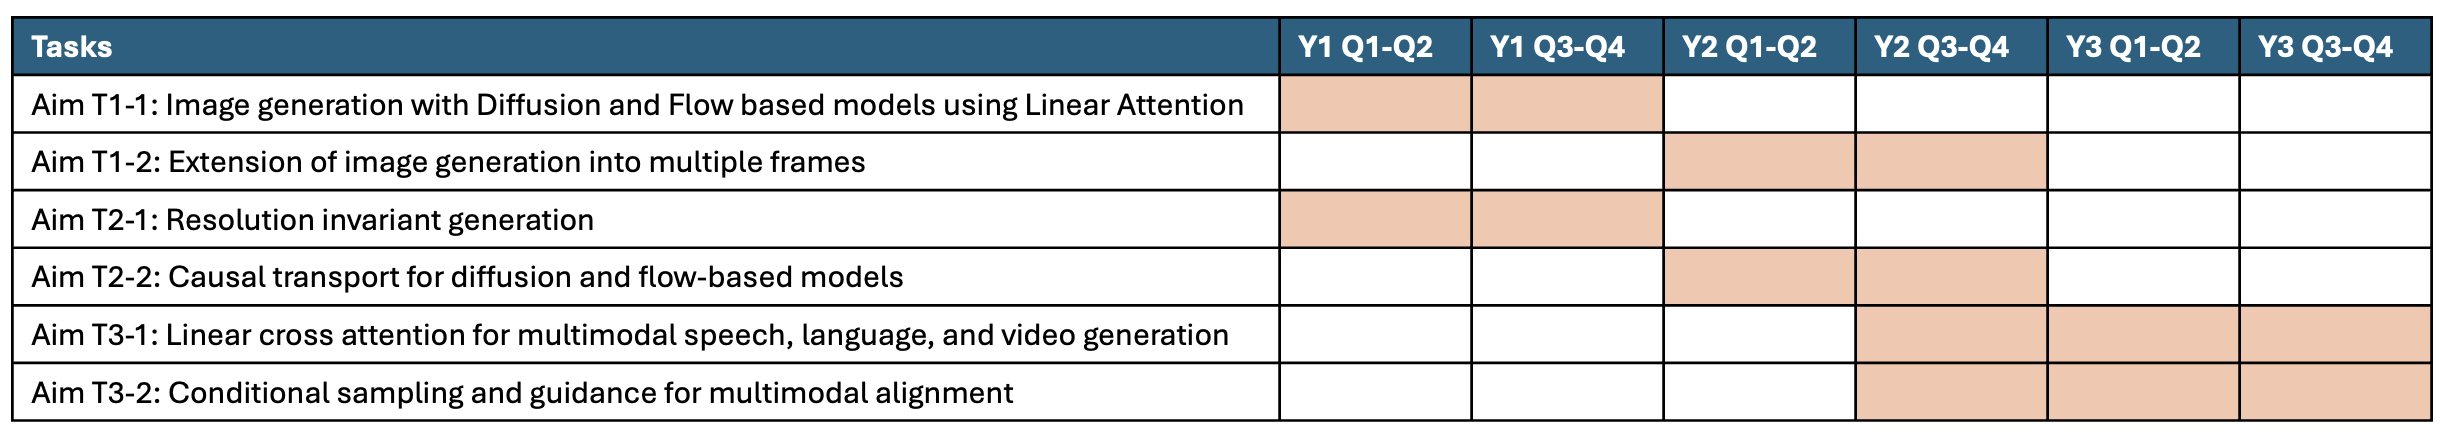
\includegraphics[width=1\textwidth]{figures/gantt.png}
\caption{Planned Project Timeline}
\label{fig:timeline}
\end{figure}

For each PI, meetings with students will take place weekly for progress, mentorship, and research support. Two doctoral students will be supported as part of this project. Joint meetings between the PIs and their respective students will take place every two weeks via Microsoft Teams. Our teams will maintain private GitHub repositories for research code and use Overleaf for joint publications. In addition to this, multiple sources of secure private cloud services are available to share data and other research documents. 


% In year 1, Aims T1-1 and T2-1 will commence immediately as the proposed advancements benefit each other but do not have strong dependencies. Work on these thrusts will continue through year 2 at which point we expect most of the proposed effort will complete. Revisions and resubmission of year 1 publications will continue in year two. Two additional papers will be submitted at the end of year 2. T3 will commence in the middle of Year 2 and will continue until completion. 

% \vspace{-1.5em}


\section*{Broader Impacts}\label{sec:BI}

\noindent\textbf{Education and workforce development:} This project will support the training of two PhD graduate students and provide an updated curriculum on generative AI development. The proposed tasks will also enable opportunities for undergraduate and masters research participation. The research is core to NSF and national security goals of advancing strategic US competitiveness, specifically in AI and accelerating AI innovation~\textbf{AI action plan citation}. The education and development of workforce is a critical piece towards this goal. 

\noindent\textbf{Addressing scaling requirements of AI: } Computational requirements of to deploy AI at scale requires significant energy, computational, and costly resources. The proposed efforts will lead to efficient and effecitve methods which will directly reduce scaling limits for broadly deploying AI. 

\noindent\textbf{Generalization to applied machine learning challenges and interdisciplinary research: } The proposed tasks are foundational to many machine learning tasks.  For example, if successful our methods can be more readily integrated into vision-language-action \cite{zitkovich2023rt} models to study physical world understanding. This would support effective and efficient operation in edge settings. Another area is for example in building personalized and local assistants. This would help protect privacy of end users.

\section*{Prior NSF Support}

PI has not received direct NSF funding and would be a first-time NSF awardee. However, PI has substantial experience contributing to externally funded research which has resulted in numerous publications at premiere venues.





% %%%
% REFERENCES
% %%%
% The References Cited section would normally begin a new page:

\clearpage
\bibliographystyle{ieee_fullname}
\bibliography{bibs/main, bibs/ding-papers, bibs/nicole-papers, bibs/video-gen, bibs/knowledge-distillation}

\setcounter{page}{1}
\newpage
\section*{Facilities, Equipment, and Other Resources}
\addcontentsline{toc}{section}{\protect\numberline{}Facilities, Equipment, and Other Resources}

The proposed project will leverage established computational and collaborative resources at Auburn University as well as shared infrastructure provided through existing interdisciplinary research centers. These resources are sufficient to support the technical and dissemination components of the proposed research. Existing collaborative mechanisms between the participating investigators, including joint research meetings and co-mentored students, will facilitate efficient coordination across sites. These resources are sufficient to support the proposed research activities without reliance on additional external facilities.

The PIs and all participating personnel will have full access to resources provided by the Department of Computer Science and Software Engineering's Assistive Intelligence Lab directed by PI Ding at Auburn University. Auburn University is designated as a National Security Agency (NSA) and Department of Homeland Security (DHS) Center of Academic Excellence in Cyber Research (CAE-R), Cyber Operations (CAE-CO), and Cyber Defense (CAE-CD). These designations reflect strengths in cybersecurity research and education and provide an established environment for interdisciplinary collaboration, graduate training, and dissemination of research outputs. The project will draw on these capabilities to support research execution and integration of results into graduate curricula and research training activities.

\noindent\textbf{Assistive Intelligence Lab:} \\
The Assistive Intelligence Lab focuses on the development of novel AI algorithms that can better understand human behaviors to facilitate naturalistic human-AI integration. The lab has approximately 8 members including PhD, MS, Undergraduate, and visitors. Auburn's CSSE department provides space and research labs for its faculty and graduate students. the Assistive Intelligence Lab occupies approximately 500 sq ft in addition to shared meeting room and facilities spaces. The CSSE department has also public access computer labs and special purpose laboratories for research. Large conference rooms are available to practice presentations and to hold meetings. Other smaller meeting rooms are also available for collaboration and discussions. High-speed wired and wireless network access is available in all areas. The CSSE department also has a dedicated server room for use by its faculty.

\noindent\textbf{Equipment:} The PI's lab has four dedicated servers are on-site which has 8xNvidia RTX 4090, 4x RTX 5090, 4x RTX PRO 6000. One additional server with 6x RTX PRO 6000 cards for development and fine tuning of deep learning models is in the department's server room. These servers are connected to 28TB of network attached storage over a 10Gbps network. Existing students also have access to multiple laptops and 2 workstations. Access to equipment will be provided via VPN.

\noindent\textbf{Alabama Supercomputer Authority (ASA): } ASA provides High Performance Computing (HPC) services at no cost to faculty, staff and enrolled students of public schools, colleges, and universities in Alabama. This allows universities to create a trained workforce with the skills needed for jobs in engineering, science, mathematics, aerospace and medical research fields. Dr. Ding and his students have been provided access to these resources. The HPC system contains 5,056 x86-64 Proc, Shared/Distributed Memory Architecture, InfiniBand high speed/low latency network, 512GB-4TB memory per node, 33 TB total memory, 1.4 PB shared storage via Panasas, A100 and H100 GPUs. 

\noindent\textbf{Office: } All faculty members have an office, and there is adequate space to host additional graduate research assistants on this project.

\noindent\textbf{Other Resources: } Departments provides the space and basic networking services to carry out the experiments, and secretarial and administrative support as well as general-purpose office equipment, such as fax, printers, and photocopiers.



\end{document}

